%\documentclass[runningheads,a4paper]{llncs}
\documentclass{llncs}

%\usepackage{amssymb}
%\setcounter{tocdepth}{3}
\usepackage{graphicx}
%\usepackage{epsfig}


%\usepackage{url}
%\urldef{\mailks}\path|sada@nii.ac.jp|

\newcommand{\comment}[1]{}
\newcommand{\Order}{\mathcal{O}}
\newcommand{\order}{o}
%\newcommand{\order}{\mathcal{o}}
\def\polylog{{\mathop{\mathrm{polylog}}\nolimits}}

\def\rank{\textit{rank}}
\def\select{\textit{select}}
\def\access{\textit{access}}
\def\pred{\textit{pred}}
\def\succ{\textit{succ}}


%%%%%%%%%%%%%%%%%%%%%%%%%%%%%%%%%%%%%%%%%%%%%%%%%%%%%%%%%%%%%%%%%%%%%%%%%%%%%%

\begin{document}

\mainmatter  % start of an individual contribution

% first the title is needed
\title{Succinct de Bruijn Graphs}

% a short form should be given in case it is too long for the running head
%\titlerunning{}

% the name(s) of the author(s) follow(s) next
%
% NB: Chinese authors should write their first names(s) in front of
% their surnames. This ensures that the names appear correctly in
% the running heads and the author index.
%
\author{
  Alexander Bowe\inst{1}
\and
  Taku Onodera\inst{2}
\and
  Kunihiko Sadakane\inst{1}
\and
  Tetsuo Shibuya\inst{2}
}

%\authorrunning{}

% the affiliations are given next; don't give your e-mail address
% unless you accept that it will be published

\institute{
  National Institute of Informatics, 2-1-2 Hitotsubashi, Chiyoda-ku, \\
  Tokyo 101-8430, Japan.
  \email{\{alex,sada\}@nii.ac.jp}
\and
  Human Genome Center, Institute of Medical Science, University of Tokyo
4-6-1 Shirokanedai, Minato-ku, Tokyo 108-8639, Japan.
  \email{\{tk-ono,tshibuya\}@hgc.jp}
}

%\date{}

%\toctitle{}
%\tocauthor{}
\maketitle
%%%%%%%%%%%%%%%%%%%%%%%%%%%%%%%%%%%%%%%%%%%%%%%%%%%%%%%%%%%%%%%%%%%%%%%%%%%%%%


\begin{abstract}
We propose a new succinct de Bruijn graph representation.  
If the de Bruijn graph of $k$-mers in a DNA sequence of length $N$ has $m$ edges,
it can be represented in $4m + \order(m)$ bits.
This is much smaller than existing ones.
The numbers of outgoing and incoming edges of a node are computed in constant time, and
the outgoing and incoming edge with given label are found in constant time
and $\Order(k)$ time, respectively.
The data structure is constructed in $\Order(Nk \log m/\log\log m)$
time using no additional space.  
\end{abstract}


%%%%%%%%%%%%%%%%%%%%%%%%%%%%%%%%%%%%%%%%%%%%%%%%%%%%%%%%%%%%%%%%%%%%%%%%%%%%%%

\def\child{\textit{outgoing}}
\def\parent{\textit{incoming}}
\def\cdeg{\textit{outdegree}}
\def\pdeg{\textit{indegree}}
\def\cedge{\textit{cedge}}
\def\search{\textit{index}}
\def\last{\textit{last}}
\def\Node{\textit{Node}}
\def\fwd{\textit{fwd}}
\def\bwd{\textit{bwd}}



\section{Introduction}
\label{sec:introduction}
Within the last two decades, assembling a genome from enormous 
amount of reads from various DNA sequencers 
has been one of the most challenging and important 
computational problems in molecular biology. 
Though the problem is proved to be NP-hard~\cite{Mye95}, 
many algorithms have been proposed for the problem (see the 
surveys~\cite{KasMor06,MilKor10,Pop09}). 
Most of these algorithms follow a so-called Overlap-Layout-Consensus strategy, 
where an algorithm first finds overlaps between reads, next layouts 
these reads, and finally finds the consensus genome. 
These algorithms can be categorized into two types, due to the graph used in 
the overlap phase. 

Most old-time assembly algorithms (especially for the long Sanger reads) 
first construct a graph called the {\it overlap graph} 
after finding the overlapping pairs of reads, 
where each node represents a read and edges are constructed between nodes 
{\it iff} the corresponding two reads have an overlap of enough 
length~\cite{BatJaf02,HuaYan05,MyeSut00}. 
But this strategy is difficult to apply against the huge data from more recent 
epoch-making next-generation sequencers (NGSs). 
The NGS machines can sequence vast amount of genome data. 
It makes it computationally very hard to compare all the pairs of reads. 
Moreover, most NGSs cannot 
read long DNA fragments ({\it e.g.}, at most 200bp in the case of Illumina HiSeq2000),  
and their read lengths are not long enough to detect overlaps with enough lengths 
between reads. 
To conquer these problems, many recent assembler algorithms utilize a graph 
called the {\it de Bruijn graph} in the overlap 
phase~\cite{LiZhu09,MacPrz09,PevTan01,SahShi12,SimWon09,ZerBir08}, 
instead of the overlap graph. 

A de Bruijn graph is a graph where each node represents a $k$-mer
(a substring of length $k$)
that exists in the reads, and an edge exists {\it iff} there is an 
exact overlap of length $k-1$ between the corresponding $k$-mers. 
The de Bruijn graph can be constructed more efficiently than the overlap graph 
in many cases, 
but the overlap phase is still the bottleneck of most assembly algorithms based 
on the de Bruijn graph. 
This is because storing the de Bruijn graph requires huge amount of memory. 
Thus we focus on reducing the memory required for the de Bruijn graph in this paper. 

There have been proposed only two data structures for
reducing the size of memory for the de Bruijn graph.
The succinct data structure proposed by Conway and Bromage~\cite{ConBro11}
is a data structure that straightforwardly
represents the de Bruijn graph by a bit vector.
Its representation should be smaller than a naive ordinary implementation of
the de Bruijn graph, but it still requires $O(m\cdot k)$ memory,
where $k$ is the $k$-mer length and $m$ is the number of edges in the de Bruijn graph,
which means it would be very large when $k$ is large.
The other data structure is by Ye et al.~\cite{YeMa12}, which
stores only a subset of nodes of the de Bruijn graph to save memory,
but it is not actually the de Bruijn graph.

In this paper, we propose a new succinct representation of a de Bruijn graph
which only requires $m(2+\log \sigma)$ bit to store\footnote{The base of logarithm is $2$.}, where
$\sigma$ is the alphabet size ({\it i.e.}, $\sigma = 4$ in the case of DNA).
The size of this representation is not affected by the value of $k$ and is
much smaller than either of the two previous methods.
Moreover we will present the algorithm to construct the data structure on-line.
Our main result is summarized as follows:
\begin{theorem}
The $k$-dimensional de Bruijn graph of $M$ string of total length $N$ on an alphabet of size $\sigma$
can be stored in $m(2+\log \sigma) + \Order((\sigma+M) \log m) + \order(m \log\sigma)$
bits where $m$ is the number of edges in the graph.  
The numbers of outgoing and incoming edges of a node are computed in $\Order(\log\sigma/\log\log m)$ time,
and the outgoing and incoming edge with given label are found in $\Order(\log\sigma/\log\log m)$ time
and $\Order(k\log^2\sigma/\log\log m)$ time, respectively.
The node for a given $k$-mer is found in $\Order(k\log\sigma/\log\log m)$ time.
If $\sigma = \polylog(m)$, the time complexities become $\Order(1)$, $\Order(1)$, $\Order(k\log\sigma)$,
and $\Order(k)$ time, respectively.
\end{theorem}

\begin{theorem}
The $k$-dimensional de Bruijn graph of a string of length $N$
can be constructed in $\Order\left(Nk \cdot \frac{\log m}{\log \log m}
(1+\frac{\log\sigma}{\log\log m})\right)$ time using no additional space.
This representation can be converted to the static one in 
$\Order\left(\frac{m\log m}{\log \log m}
(1+\frac{\log\sigma}{\log\log m})\right)$ time.
\end{theorem}
For DNA sequences ($\sigma=4$), the succinct de Bruijn graph can be constructed in 
$\Order(Nk \log m/\log\log m)$ time and its space becomes $4m + \order(m)$ bits.
This is much smaller than existing ones.
For example, the succinct representation of Conway and Bromage~\cite{ConBro11}
uses 40.8GB for storing a de Bruijn graph with $m = $ 12,292,819,311 edges
and $k = 27$ (28.5 bits per edge).  
On the other hand, if we use an efficient implementation
of {\rank}/{\select} data structures~\cite{OkaSad07} for our representation,
the estimated size is less than $5$ bits per edge.  
Therefore the above graph is stored in less than 8GB.


%%%%%%%%%%%%%%%%%%%%%%%%%%%%%%%%%%%%%%%%%%%%%%%%%%%%%%%%%%%%%%%%%%%%%%%%%%%%%%

\section{Preliminaries}\label{sec:preliminaries}

\subsection{de Bruijn graphs}
In the original definition~\cite{deBruijn46}, the $k$-dimensional de Bruijn graph of $\sigma$ symbols
is a directed graph representing overlaps between strings of symbols defined as follows.
The graph has $\sigma^k$ nodes, consisting of all length-$k$ strings of the symbols.
A node is denoted by $(u_1,\ldots,u_k)$ where $u_1,\ldots,u_k$ are symbols.
For any pair of nodes $u = (u_1,\ldots,u_k)$ and $v = (v_1,\ldots,v_k)$ 
such that 
$u_2 = v_1, u_3 = v_2, \ldots, u_k = v_{k-1}$, the graph has a directed
edge from $u$ to $v$ labeled with $v_k$.
In this paper we call it the complete $k$-dimensional de Bruijn graph
of $\sigma$ symbols.

The de Bruijn graphs considered in this paper are subgraphs of the complete de Bruijn graph.
We define the $k$-dimensional de Bruijn graph of a string $T$ as follows.
The nodes of the graph correspond to all length-$k$ substrings of $T$.  If the string is of length $N$,
the graph has at most $N-k+1$ nodes.  The edges of the graph are defined in the same way as the complete
de Bruijn graph.  For convenience, we add $k$ characters \$ at the head of the string,
and a \$ at the end.

We can also store a set of $M$ strings $T_1,\ldots,T_M$ as follows.
We append a terminator $\$_i$ to the tail of each string $T_i$,
and concatenate all the strings.  Then we add $k$ characters $\$_0$ at the head.
Figure~\ref{fig:debruijn} shows an example.


%dummy node���lj�����


\begin{figure}[bt]
\begin{center}
  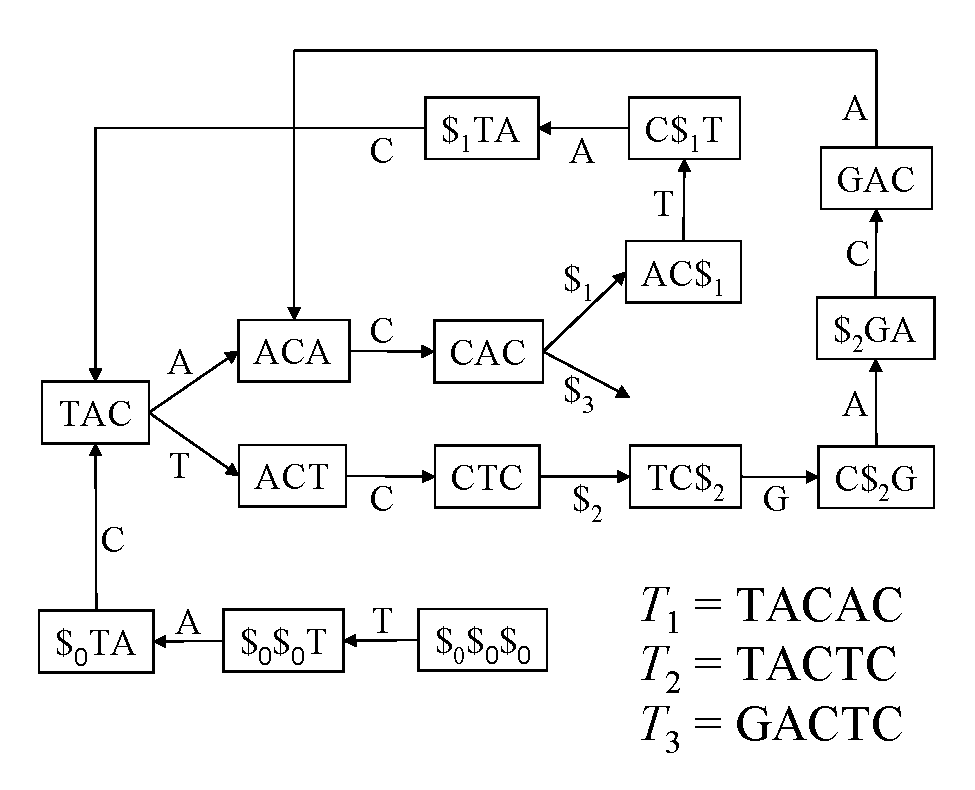
\includegraphics[scale=0.70]{fig3.eps}
\caption{The $3$-dimensional de Bruijn graph of strings `TACAC', `TACTC', and
`GACTC'.}
\label{fig:debruijn}
\end{center}
\end{figure}

\subsection{Basic succinct data structures}\label{sec:rank}

Let $T = T[1] T[2] \cdots T[N]$ be a string of length $N$ on alphabet ${\cal A}$,
that is, $T[i] \in {\cal A}$ for any $i=1,\ldots,N$.
Let $\sigma = |{\cal A}|$ denote the alphabet size.
We can store $T$ in $N \lceil \log_2 \sigma \rceil$ bits.  The space does not
depend on the word size of CPU.  We can retrieve any character $T[i]$ in constant
time using bit operations on words.

The most basic succinct data structure is the one for computing {\rank}, {\select}, and {\access}
values on strings, which are defined as follows.
The value ${\access}(T,i)$ returns $T[i]$ for $1 \le i \le N$.
The value ${\rank}_c(T,i)$ where $c \in {\cal A}$ and $1 \le i \le N$
is the number of $c$'s in $T[1] \cdots T[i]$.  For any $T$ and $c$ we define
${\rank}_c(T,0) = 0$.
The value ${\select}_c(T,j)$ where $c \in {\cal A}$ and $1 \le j \le {\rank}_c(T,N)$
is the position of $j$-th $c$ in $T$.
For any $T$ and $c$ we define ${\select}_c(T,0) = 0$ and for any $j > {\rank}_c(T,N)$
${\select}_c(T,j) = N+1$.
Let $t_r(N,\sigma)$, $t_s(N,\sigma)$, and $t_a(N,\sigma)$ denote the time complexity for computing
{\rank}, {\select}, and {\access}, respectively, on a string of length $N$ and alphabet size $\sigma$.
For brevity, we assume that 
for any $N_1 \le N_2$, $t_r(N_1,\sigma) \le t_r(N_2,\sigma)$ and
for any $\sigma_1 \le \sigma_2$, $t_r(N,\sigma_1) \le t_r(N,\sigma_2)$.
Let $t_b(N,\Sigma)$ denote the maximum of 
$t_r(N,\sigma),t_s(N,\sigma),t_a(N,\sigma)$.

For convenience, we define ${\pred}_c(T,i) = {\select}_c(T, {\rank}_c(T, i))$
which is the position of the first occurrence of $c$ when we scan $T$ from the position $i$ to the head,
and ${\succ}_c(T,i) = {\select}_c(T, {\rank}_c(T, i-1)+1)$
which is the position of the first occurrence of $c$ when we scan $T$ from the position $i$ to the end.
If $T[i]$ is the first (last) occurrence of $c$, {\pred} (\succ) returns $0$ ($N+1$).

%From the definition it holds that
%${\select}_c(T, {\rank}_c(T, i)) \le i$ for any $1 \le i \le n$ and
%${\rank}_c(T, {\select}_c(T, j)) = j$ for any $1 \le j \le {\rank}_c(T,n)$.

There exist many succinct data structures for {\rank} and {\select} on strings.
Among them, we use the one by Ferragina et al.~\cite{FerManMakNav06} for the static case
(the case the string does not change).  A string of $T$ length $n$ on an alphabet of size $\sigma$
can be stored in $nH_0(T) + \Order(\sigma \log n) + \order(n \log\sigma)$ bits so that
{\rank}, {\select} and {\access} queries take $\Order(\log\sigma / \log\log n)$ time,
where $H_0(T)$ denotes the order-$0$ entropy of the string.  Note that if the alphabet size $\sigma$
is $\polylog(n)$, the queries are done in constant time.  For a binary alphabet case,
we can use a simpler data structure that has the same time and space complexities~\cite{RRR07}.

For the dynamic case where the string is modified by inserting or deleting a character,
we use the one by Navarro and Sadakane~\cite{NavSad10} which stores the string
in $nH_0(T) + \Order(\sigma \log n) + \order(n \log\sigma)$ bits so that
{\rank}, {\select} and {\access} queries and insertion and deletion of a character take
$\Order(\frac{\log n}{\log \log n}(1+\frac{\log\sigma}{\log\log n}))$ time.
For polylog-sized alphabets, the operations are done in optimal $\Order(\log n/\log \log n)$ time.
The time complexities for insert and delete are denoted by $t_u(n,\sigma)$.


\subsection{The XBW data structure}
The XBW-transform~\cite{FLMM09} is a method for compressing and indexing labeled trees.
It is an extension of the Burrows-Wheeler transform~\cite{BurWhe94} used for compressing
and indexing strings.  Given a rooted tree with $n$ nodes where each node has a label in
the set of size $\sigma$, the XBW-transform converts the tree into a representation of
$2n + n \log\sigma$ bits.  The size of the representation matches the information-theoretic
lower bound.  We can support tree navigational operations by adding small-size auxiliary
indexes.

Because the XBW is for storing a tree, we cannot use it directly for storing de Bruijn graphs,
which is a cyclic graph.
This paper proposes a new compact representation of de Bruijn graphs of strings.


%%%%%%%%%%%%%%%%%%%%%%%%%%%%%%%%%%%%%%%%%%%%%%%%%%%%%%%%%%%%%%%%%%%%%%%%%%%%%%

\section{Succinct de Bruijn Graphs}\label{sec:sdg}

Let $G$ be a $k$-dimensional de Bruijn graph of a string $T$ of length $N$ on alphabet ${\cal A}$.
Let $n$ and $m$ be the numbers of nodes and edges of $G$, respectively.
A succinct representation of $G$ supports the following operations:
\begin{itemize}
\item ${\cdeg}(v)$ returns the number of outgoing edges from node $v$.
%\item ${\cedge}(v, i)$ 
%\item ${\child}(v, i)$ returns the node $w$ pointed to by the $i$-th outgoing edge of node $v$
%($1 \le i \le {\cdeg}(v)$).
\item ${\child}(v, c)$ returns the node $w$ pointed to by the outgoing edge of node $v$
with edge label $c$.  If no such node exists, it returns $-1$.
\item ${\pdeg}(v)$ returns the number of incoming edges to node $v$.
%\item ${\parent}(v, i)$ returns the node $w$ that is on the $i$-th incoming edge of node $v$
%($1 \le i \le {\pdeg}(v)$).
\item ${\parent}(v, c)$ returns the node $w = (w_1,\ldots,w_k)$ such that 
there is an edge from $w$ and $v$
and $w_1 = c$.  If no such node exists, it returns $-1$.
\item ${\search}(s)$ returns the index $i$ of the node whose label is the string $s$ of length $k$.
%Precisely, $i$ such that ${\last}[i] = 1$ and ${\Node}[i] = s$.
\end{itemize}

We define ${\cal A}^-$ as any set of size $|{\cal A}|$ such that ${\cal A}^- \cap {\cal A} = \emptyset$.
Let $c^-$ denote an element of ${\cal A}^-$ corresponding to an element $c \in {\cal A}$.
We also define a function $u$ as $u(c^-) = c$ for any $c^- \in {\cal A}^-$
and $u(c) = c$ for any $c \in {\cal A}$.  We assume that the function is evaluated in constant time.

\subsection{The succinct representation}

The representation consists of the following components:
\begin{itemize}
\item a string $W = W[1] W[2] \cdots W[m]$ where each character is from ${\cal A} \cup {\cal A}^-$.
\item a string ${\last}$ of length $m$ on the binary alphabet $\{0,1\}$.
\item an array $F$ of length $\sigma = |{\cal A}|$.
\end{itemize}
An example is shown in Figure~\ref{fig:succinctdebruijn}.

The string $W$ is defined as follows.
Each character $W[i]$ represents the label of an edge of $G$.
Each edge $u \rightarrow v$ of $G$ is associated with the node label of $u$.
Those edge labels are sorted in the lexicographic order of reversals of associated node labels.
Ties are broken by edge labels.
Let ${\Node}[i]$ denote the node label for $W[i]$.  This is not explicitly stored.

The string ${\last}$ is defined as
${\last}[i] = 1$ if $i = n$ or ${\Node}[i]$ is different from ${\Node}[i+1]$,
or ${\last}[i] = 0$ otherwise.  From this definition,
all node labels ${\Node}[i]$ with ${\last}[i] = 1$ are distinct, and
those indices $i$ have one-to-one correspondence with the nodes of $G$.
Therefore we use an index $i$ of the strings such that ${\last}[i] = 1$
to represent a node $v$.  
%There are $n$ such indices.
Let $n$ denote the number of nodes.

The array $F$ stores cumulative frequencies of the last characters of node labels.
Namely, for any $c \in {\cal A}$, 
%$F[c] = |\{i \mid 1 \le i \le m, \mbox{the last character of ${\Node}[i]$ is
%smaller than $c$}  \}|$
$F[c] = |\{i \mid 1 \le i \le m, C(i) < c  \}|$
where $C(i)$ denotes the last character of ${\Node}[i]$.
Because $F[\$_i] = i$ for $i = 0,1,\ldots,M$, we need not store them.

The array $F$ is represented in $\Order(\sigma \log m)$ bits.
If $F$ does not change, we can store it as it is using a simple array and $F[c]$ is computed
in constant time.
In a dynamic case that a new node or edge is inserted to the de Bruijn graph,
we have to update $F$ accordingly.  By using a balanced binary tree, $F$ can be maintained
in $\Order(\log \sigma)$ time.

We also use the inverse of $F$, that is, given $i$, we need to know the last character $c$
of ${\Node}[i]$.  In a static case, this can be
computed in constant time using a {\rank}/{\select} data structure of
$\Order(\sigma \log m) + \Order(m \log\log m/\log m)$ bits~\cite{RRR07}.
In a dynamic case, it is done in $\Order(\log \sigma)$ time using a balanced
binary search tree.
%
It can be improved to $\Order(\frac{\log m }{\log \log m}
(1+\frac{\log\sigma}{\log\log m}))$ time using \cite{NavSad10}.
This data structure uses
$\Order(\sigma \log n) + \Order(m \log \log m/\log m)$ bits.
%
Let $t_f$ denote the largest time complexity of those operations.


\begin{figure}[bt]
\begin{center}
  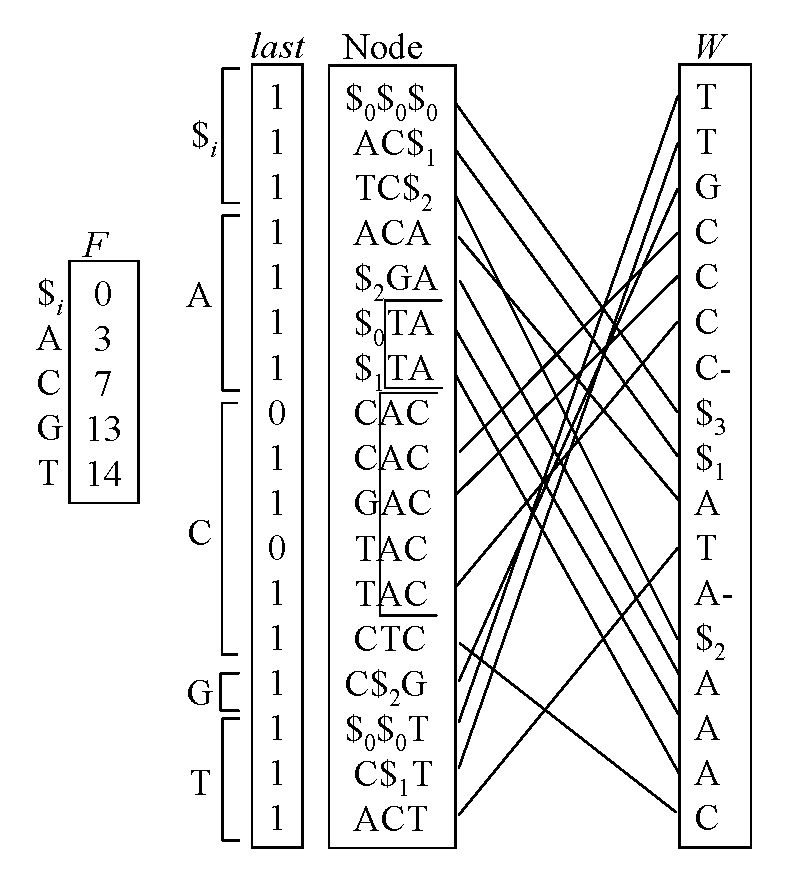
\includegraphics[scale=0.70]{fig4.eps}
\caption{The succinct representation of the de Bruijn graph in Figure~\ref{fig:debruijn}.
Lines between {\Node} and $W$ show {\fwd} and {\bwd} functions.
}
\label{fig:succinctdebruijn}
\end{center}
\end{figure}


A character $W[i]$ is from either ${\cal A}$ or ${\cal A}^-$.
If $W[i]$ is from ${\cal A}^-$, it means that there exists $j < i$ such that
$W[j] = u(W[i])$ and ${\Node}[j]$ and ${\Node}[i]$ have the identical suffix of length $k-1$.

We can define a one-to-one mapping between indices $i$ of ${\last}$ with ${\last}[i] = 1$
and indices $j$ of $W$ with $W[j] \in {\cal A}$.
As stated above, the indices $i$ with ${\last}[i] = 1$ have one-to-one correspondence with
the nodes of the de Bruijn graph $G$.  Consider indices $j$ with $W[j] \in {\cal A}$.
Let ${\Node}^\prime[j]$ denote
the concatenation of the length $k-1$ suffix of ${\Node}[j]$ and $W[j]$.
For any ${\Node}^\prime[j]$, there exists $i$ such that ${\Node}[i] = {\Node}^\prime[j]$.
Because of the definition of $W$, there are no indices $j$ and $j^\prime$ 
($j \neq j^\prime$) such that ${\Node}^\prime[j] = {\Node}^\prime[j^\prime]$.
Therefore there is a one-to-one mapping.  Furthermore, the mapping is represented by
{\rank} and {\select} queries on $W$.
Let $i,j$ be indices such that ${\last}[i] = 1$ and ${\Node}[i] = {\Node}^\prime[j]$.
Let $c = C(i)$ be the last character of ${\Node}[i]$ and 
$r = {\rank}_1({\last}, i) - {\rank}_1({\last}, F[c])$.
Then it holds $j = {\select}_c(W, r)$.  
From $j$, $i$ is computed by $c = W[i]$, $r = {\rank}_c(W, j)$ and
$i = {\select}_1({\last}, {\rank}_1({\last}, F[c]) + r)$.
We define $\bwd(i) = j$ and $\fwd(j) = i$.
The time complexities of $\bwd(i)$ and $\fwd(j)$ are
$\Order(t_f + t_b(m,2\sigma))$.

%Note that the function ${\bwd}(i^\prime)$ for ${\last}[i^\prime] = 0$
%returns the same value as ${\bwd}(i)$ where $i$ is the index such that
%${\last}[i] = 1$ and ${\Node}[i^\prime] = {\Node}[i]$.

Our data structure is similar to the XBW data structure~\cite{FLMM09} in the sense
that the {\last} array in ours is the same as $S_{\last}$ in the XBW.
We propose a new encoding scheme for storing labels of a graph.


\subsection{The {\cdeg} and {\child} operations}
The ${\cdeg}(v)$ operation is easy to support.
We assume that $v$ is the index of ${\last}$ such that ${\last}[v] = 1$ and
${\Node}[v]$ is the label of the node.
From the definition of ${\last}$, it is obvious that 
${\cdeg}(v) = v - {\pred}_1({\last}, v-1)$.
The time complexity is $\Order(t_b(m,2))$.

The ${\child}(v,c)$ operation is done as follows.
For any $1 \le i \le m$, we define $R(i) = [{\pred}_1({\last},i-1)+1,{\succ}_1({\last},i)]$,
which is the range of $W$ and ${\last}$ that for all $j \in R(i)$, ${\Node}[j]$ are identical.
The labels of outgoing edges of node $v$ are stored in $W[j]$ for $j \in R(v)$.
%and they are sorted.  
%
%binary search�����Ȃ��Ă��Crank/select�ł����Ȃ苁�܂��D
%We perform a binary search in the range using the ${\access}$ operation
%on $W$.  Note that during the binary search we regard any character $a^- \in {\cal A}^-$
%as the corresponding character $a$ in ${\cal A}$.
Let $j$ be the index such that $u(W[j]) = c$.
We can find $j$ by ${\pred}_c(W, v)$ and ${\pred}_{c^-}(W, v)$.
Then $x = {\child}(v,c)$ can be computed by $x = \fwd(j)$.

The time complexity for ${\child}(v,c)$ is 
$\Order(t_f + t_b(m, 2\sigma))$.

\subsection{The {\pdeg} and {\parent} operations}
Consider to compute ${\pdeg}(v)$.
Let $d = C(v)$ and $x = bwd(v)$.  Then it holds $d = W[x]$ and the first character
of ${\Node}[x]$ is the label of an edge pointing to $v$.
Let $y = {\succ}_d(W, x)$.  Then all $d^-$ between $W[x]$ and $W[y]$ correspond
to parents of $v$.  The number of such $d^-$ is computed by {\rank} on $W$.
The time complexity is $\Order(t_f + t_b(m,2\sigma))$.

To compute ${\parent}(v,c)$, we need to obtain the first character of ${\Node}[i]$
such that $x \le i < y$ and $u(W[i]) = d$.  The first character of ${\Node}[i]$
is computed by $C(b^{k-1}(i))$ where $b^{k-1}$ stands for applying
${\bwd}({\succ}_1({\last},i))$ repeatedly $k-1$ times.  
We perform a binary search to
find the index $i$ such that $c = C({\bwd}^{k-1}(i))$.
The time complexity is 
$\Order(k(t_f + t_b(m,2\sigma))\log\sigma)$.

\subsection{The {\search} operation}
Recall that ${\search}(s)$ returns the index $i$ of the node whose label 
is the string $s$ of length $k$.
Precisely, it returns $i$ such that ${\last}[i] = 1$ and ${\Node}[i] = s$.
The algorithm for ${\search}(s)$ is similar to \cite{FerMan05}.
Let $i_1 < i_2 < \cdots < i_w$ be the indices such that
${\last}[i_j] = 1$ and ${\Node}[i_j]$ and $s$ have the same suffix of length $d$ ($1 \le d \le k$).
Let $i_0$ be the smallest index in $R(i_1)$.
Then for any $i$ such that $i_0 \le i \le i_w$, ${\Node}[i]$ and $s$ have the same suffix of length $d$
and for other indices this does not hold.
Therefore ${\search}(s)$ can be done by computing 
ranges $[i_0, i_w]$ for $d = 1,2,\ldots,k$.
Let $c_d$ denote the $d$-th character of $s$ ($1 \le d \le k$).
For $d=1$, the range is $[F[c_1]+1, F[c_1+1]]$.
Given the range $[\ell_d, r_d]$ for $d$,  we can compute the range $[\ell_{d+1}, r_{d+1}]$ for $d+1$
as follows.  The end of the range $r_{d+1}$ is computed by $r_{d+1} = {\child}(r_d, c_{d+1})$.
The beginning of the range $\ell_d$ is computed by ${\pred}_1({\last},{\child}({\succ}_1({\last}, \ell_d), c_{d+1})+1$.

The above algorithm can be simplified.  Instead of computing ranges $[i_0, i_w]$,
we can use $[i_1, i_w]$.  For $d=1$, the range is $[{\succ}_1({\last},F[c_1]+1), F[c_1+1]]$.
Given the range $[\ell_d, r_d]$ for $d$, the range for $d+1$ is obtained by
$r_{d+1} = {\child}(r_d, c_{d+1})$ and $\ell_{d+1} = {\child}(\ell_d, c_{d+1})$.
The time complexity is $\Order(k(t_f + t_b(m,2\sigma)))$.

\subsection{Time and space complexities}
We implement the above data structure for the static case using known succinct data structures.
The array $F$ is stored in $\sigma \log m$ bits.  The data structure for computing $C(i)$
uses $\Order(\sigma \log m) + \Order(m \log \log m/\log m)$ bits.  The operation time $t_f$ is constant.
The string {\last} is stored in $m+\order(m)$ bits so that {\rank}, {\select}, and {\access} takes constant 
time~\cite{RRR07}.  The string $W$ is stored by using \cite{FerManMakNav06}.  
Because the characters
of $W$ are from ${\cal A} \cup {\cal A}^- \cup \{\$_1,\ldots,\$_M\}$, 
the alphabet size is $2\sigma + M$.
%
%Note that there is another character \$ in $W$ which indicates the end of the string, but
%we do not encode it in $W$.  Instead we store the position of the character using $\log m$ bits.
%Then the alphabet size of $W$ is $2\sigma$.  
We can reduce the alphabet size to $2\sigma+1$ by unifying the $M$ terminators
$\$_1,\ldots,\$_M$ into a character \$.  We distinguish two terminators, but
encode them using the same code.

The string $W$ is stored in $m \log (2\sigma+M) +
\Order((\sigma+M) \log m) + \order(m \log\sigma)
 = m + m \log\sigma + \Order((\sigma+M) \log m) + \order(m \log\sigma)$ bits,
and the time complexities $t_r, t_s, t_a$ are 
$\Order(\frac{\log\sigma}{\log\log m})$.
Therefore the time complexities for {\cdeg}, {\pdeg}, {\child}, {\parent},
and {\search} are $\Order(\frac{\log\sigma}{\log\log n})$, 
$\Order(\frac{\log\sigma}{\log\log n})$, 
$\Order(\frac{\log\sigma}{\log\log n})$, 
$\Order(\frac{k\log^2\sigma}{\log\log n})$,
$\Order(\frac{k\log\sigma}{\log\log n})$, respectively.

For polylog-size alphabets, {\cdeg}, {\pdeg} and {\child} takes constant time,
{\parent} takes $\Order(k \log \sigma)$ time,
and {\search} takes $\Order(k)$ time.


%%%%%%%%%%%%%%%%%%%%%%%%%%%%%%%%%%%%%%%%%%%%%%%%%%%%%%%%%%%%%%%%%%%%%%%%%%%%%%

\section{On-line construction}
In this section we propose an on-line construction algorithm of the de Bruijn graph of a string.
Here on-line means given the succinct de Bruijn graph $G$ of a string $T = T[1] \cdots T[N]$, we change it
to the succinct de Bruijn graph $G^\prime$ of the string $T^\prime = T[1] \cdots T[N+1]$ which is made by
appending a character to $T$.
%We give two algorithms; one is space-efficient and the other is faster.
%The former uses no additional space, while the latter uses ..............................
%
%\subsection{Space-efficient algorithm}

As stated above, our succinct representation of $G$ assumes that a character \$ is appended
to the end of $T$.  Let $p$ be the position of \$ in $W$.
To construct the succinct representation of $G^\prime$,
we first change $W[p]$ from \$ to $T[N+1]$ and modify other parts if necessary,
then insert \$ to another position of $W$.  The details are as follows.

Let $p$ be the position of \$ in $W$ for the string $T = T[1] \cdots T[N]$.
If a new character $c = T[N+1]$ is appended to the end of $T$, we change $W[p]$ from \$ to $T[N+1]$.
We have to maintain the invariant that for all $i \in R(p)$, that is, ${\Node}[i] = {\Node}[p]$,
$W[i]$ are distinct.
% and sorted alphabetically.  
%Such $i$'s satisfy
%$p \le i \le {\succ}_1({\last}, p)$.  We do a binary search in this range to find the correct
%position $p^\prime$ for $T[N+1]$.  
Because before changing $W[p]$ they are distinct, we can check the invariant by finding the character
$c = T[N+1]$ or $c^-$ in $W[i]$ such that $i \in R(p)$.  This is done by {\rank} and {\select} on $W$.
%If the same character as $T[N+1]$ does not exist in the range, 
%we insert $T[N+1]$ at the beginning of the range.  Let $x$ denote this position.
%otherwise we do not insert and we delete $W[p]$ and ${\last}[p]$.

If $T[N+1]$ already exists in the range, let $p^\prime$ be its position.
We delete $W[p]$ and ${\last}[p]$ and we insert \$ in $W$ at position $x = {\fwd}(p^\prime)$.
We also insert $0$ in ${\last}[x]$ because ${\Node}[x]$ already exists.
We update $p = x$ and the array $F$ accordingly.

If $T[N+1]$ does not exist in the range,
we change $W[p] = \$ $ to either $c = T[N+1]$ or $c^-$.
To determine $c$ or $c^-$, we first find the nearest occurrence of $c$ to $W[p]$,
namely, its position is $j = {\pred}_c(W, p-1)$ if it exists ($j > 0$).
We compare ${\Node}[j]$ with ${\Node}[p]$.  If they have the same suffix of length $k-1$,
we change $W[p]$ to $c^-$, and otherwise change $W[p]$ to $c$.
We compare characters of ${\Node}[j]$ and ${\Node}[p]$ one by one using the {\bwd} function.
We also compare ${\Node}[j_2]$ with ${\Node}[p]$ where
$j_2 = {\succ}_c(W, p+1)$ if it exists ($j_2 \le m$).
If they share the length $k-1$ suffix, we change $c_2 = W[j_2]$ to $c_2^-$.
This takes $\Order(k(t_f + t_b(m,2\sigma)))$ time.
If the nearest $c$ does not exist ($j = 0$), let $j = F[c]$.
The position $x$ to insert \$ is computed by $x = {\fwd}(j)$.
We insert $0$ to ${\last}[x]$ if $W[p]$ or $W[j_2]$ has a character in ${\cal A}^-$,
or $1$ otherwise.  Finally we set $p = x$ and update the array $F$.

In total, the update operation takes 
$\Order(k(t_f + t_b(m,2\sigma)))$ time.
If we use the dynamic {\rank}/{\select} data structure of \cite{NavSad10}
for $W$ and ${\last}$, $t_b = \Order(\frac{\log m}{\log \log m}(1+\frac{\log\sigma}{\log\log m}))$ time.
We also use \cite{NavSad10} for computing $C(i)$.  Then $t_f = \Order(\frac{\log m }{\log \log m}(1+\frac{\log\sigma}{\log\log m}))$
and the space is $\Order(\sigma \log n) + \Order(m \log \log m/\log m)$ bits.
Because we repeat this update operation $N$ times for all characters of the input string,
the succinct de Bruijn graph can be constructed in
$\Order\left(Nk \cdot \frac{\log m}{\log \log m}
(1+\frac{\log\sigma}{\log\log m})\right)$ time.
For polylog-sized alphabets, it becomes $\Order(Nk \cdot \frac{\log m}{\log \log m})$.

It is easy to construct the static data structure from the dynamic one.
The strings {\last} and $W$ for the static one are generated by
applying {\access} operations to the dynamic one for $i=1,\ldots,m$
in $\Order(m t_b(m,2\sigma))$ time.
After constructing the static strings, the auxiliary data structures for
computing {\rank}/{\select} are constructed in $\Order(m)$ time.

%%%%%%%%%%%%%%%%%%%%%%%%%%%%%%%%%%%%%%%%%%%%%%%%%%%%%%%%%%%%%%%%%%%%%%%%%%%%%%

\section{Concluding remarks}\label{sec:conclusion}
We have proposed a succinct representation of de Bruijn graphs,
which can be constructed with efficient time and space complexities,
and in an on-line manner.
Therefore they are useful for large-scale genome assembly.

The succinct de Bruijn graph can be also used for data compression.
The PPM (Prediction by Partial Matching) is a text compression algorithm~\cite{CleWit84}.
In the order-$k$ PPM, a character is compressed using statistical information
that it appears after a string of length $k$ based on a given probability distribution.
We can easily extend our succinct de Bruijn graph to be used for PPM compression.
In addition to the array $W$, we use another array to store the numbers of times
that each edge is traversed.  Then we have enough information for compression.
The succinct de Bruijn graph is used for natural language processing because
it stores all $n$-grams in a text.

Our future work will be to improve the time complexity for the on-line construction
algorithm, and to implement the proposed data structure and apply it
for assembling large genomes and PPM data compression.
A sample source code is available at {\tt http://code.google.com/p/csalib/}.


%%%%%%%%%%%%%%%%%%%%%%%%%%%%%%%%%%%%%%%%%%%%%%%%%%%%%%%%%%%%%%%%%%%%%%%%%%%%%%

\subsection*{Acknowledgments}
KS and TS are supported in part by KAKENHI 23240002.

%%%%%%%%%%%%%%%%%%%%%%%%%%%%%%%%%%%%%%%%%%%%%%%%%%%%%%%%%%%%%%%%%%%%%%%%%%%%%%
%%%%%%%%%%%%%%%%%%%%%%%%%%%%%%%%%%%%%%%%%%%%%%%%%%%%%%%%%%%%%%%%%%%%%%%%%%%%%%

\bibliographystyle{plain}
\bibliography{intro}

%%%%%%%%%%%%%%%%%%%%%%%%%%%%%%%%%%%%%%%%%%%%%%%%%%%%%%%%%%%%%%%%%%%%%%%%%%%%%%
%%%%%%%%%%%%%%%%%%%%%%%%%%%%%%%%%%%%%%%%%%%%%%%%%%%%%%%%%%%%%%%%%%%%%%%%%%%%%


\end{document}

